\documentclass{atistandalonetask}
\usepackage{atistandard}
\begin{document}
	  \begin{atiTask}[
  title = Volumen eines Schwimmbeckens
  %call = Zusatzaufgabe,
	]
In einem Schwimmbad befinde sich ein Becken mit der in Abbildung 1 wiedergegebenen Grundfläche (mit Blick aus der $z$-Richtung). Die Wassertiefe sei gleichförmig zunehmend mit der Funktion $z(x,y)=\frac{1}{10}\cdot y$. Berechnen Sie das Wasservolumen durch Ausführen von Mehrfachintegralen.\\[-0.7cm]
\begin{figure}[h]
\centering
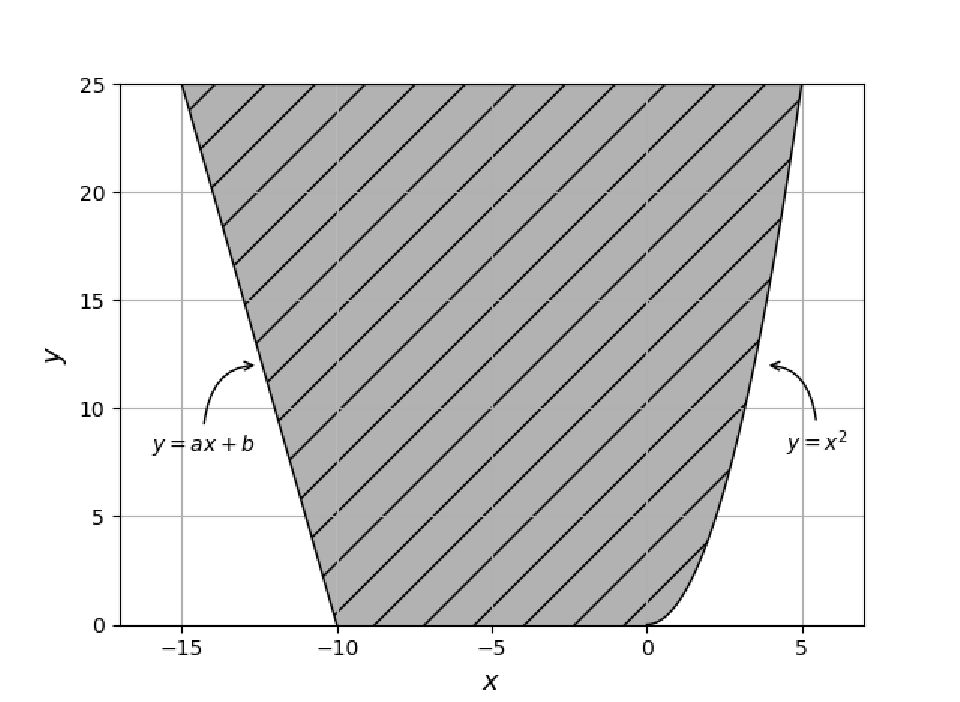
\includegraphics[width=0.7\linewidth]{./picture-dreifachintegral}
%\caption{}
\label{fig:picture-dreifachintegral}
\end{figure}


\atiNote{Bestimmen Sie die Konstanten $a$ und $b$ aus der Skizze.}
\end{atiTask}

 \begin{atiSolution}
   	Lösung folgt
  	%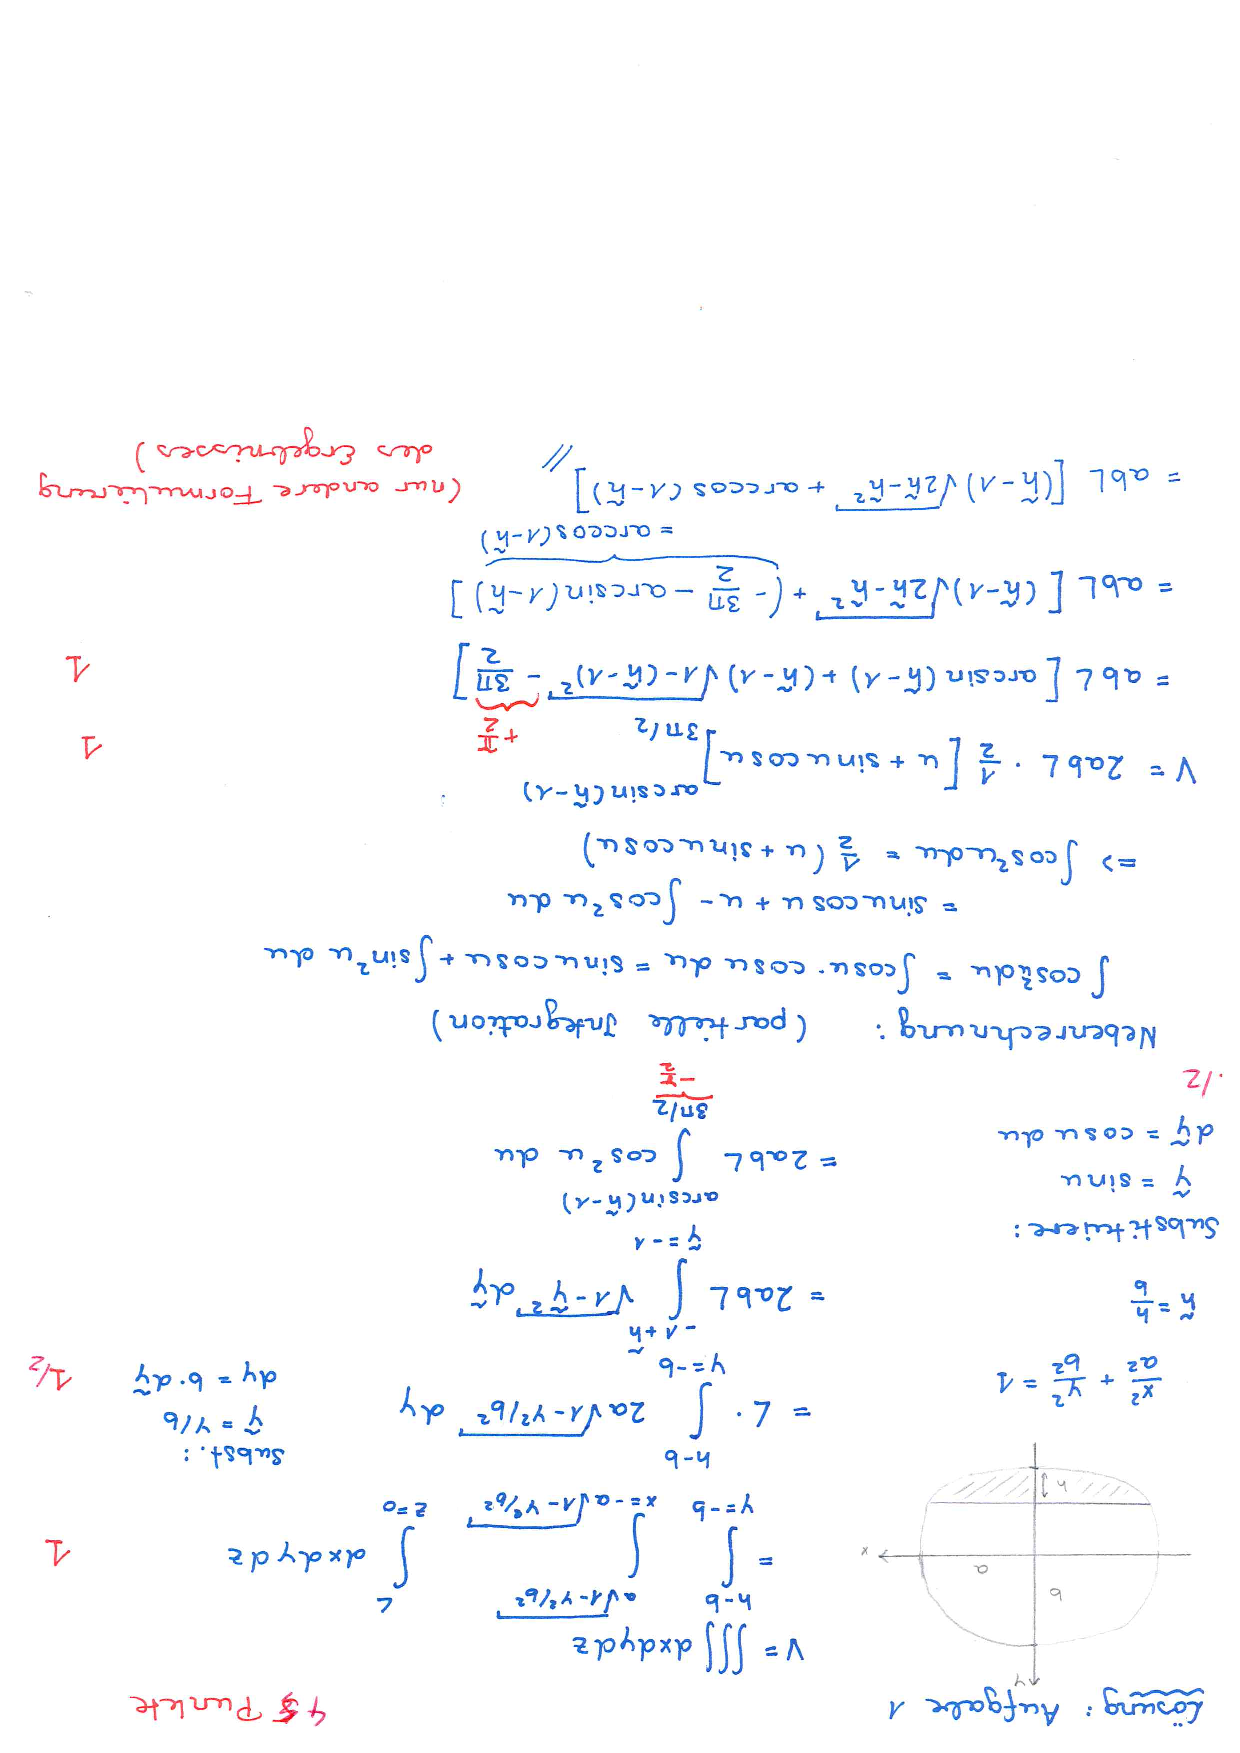
\includepdf[pages=-]{solution-doppelintegral_iii.pdf}
  \end{atiSolution}
\end{document}